\documentclass[11pt]{article}


    \usepackage[breakable]{tcolorbox}
    \tcbset{nobeforeafter} % prevents tcolorboxes being placing in paragraphs
    \usepackage{float}
    \floatplacement{figure}{H} % forces figures to be placed at the correct location
    \usepackage{multicol}
	\usepackage[english]{babel}
    \usepackage{tabularx}
    \usepackage{subfigure}
    \usepackage{picture}
    \usepackage{amsmath}
    \usepackage{hyperref}
    \hypersetup{
    colorlinks=true,
    linkcolor=blue,
    filecolor=magenta,      
    urlcolor=cyan,
    }
    \usepackage{graphicx}    
    \usepackage{caption}
    \usepackage{adjustbox} % Used to constrain images to a maximum size 
    \usepackage{xcolor} % Allow colors to be defined
    \usepackage{enumerate} % Needed for markdown enumerations to work
    \usepackage{geometry} % Used to adjust the document margins
    \usepackage{amsmath} % Equations
    \usepackage{amssymb} % Equations
    \definecolor{urlcolor}{rgb}{0,.145,.698}
    \definecolor{linkcolor}{rgb}{.71,0.21,0.01}
    \definecolor{citecolor}{rgb}{.12,.54,.11}
    

    
    % Prevent overflowing lines due to hard-to-break entities
    \sloppy 
    % Setup hyperref package
    \hypersetup{
      breaklinks=true,  % so long urls are correctly broken across lines
      colorlinks=true,
      urlcolor=urlcolor,
      linkcolor=linkcolor,
      citecolor=citecolor,
      }
    % Slightly bigger margins than the latex defaults
    
    \geometry{verbose,tmargin=1in,bmargin=1in,lmargin=0.4in,rmargin=1in}
    \usepackage{fancyhdr}
    \pagestyle{fancy}
    \renewcommand{\footrulewidth}{1pt}
    \rhead{e11921655 Fabian Holzberger \\ e01526208 Jan Ellmenreich}
    \lhead{VU\,184.725\\ High Performance Computing}
    \cfoot{\thepage}
    \setcounter{secnumdepth}{0}
    \setlength\parindent{0pt}

    \usepackage{booktabs}

    \usepackage{listings}
    \usepackage[linesnumbered,ruled,vlined]{algorithm2e}
    \newcommand\mycommfont[1]{\footnotesize\ttfamily\textcolor{blue}{#1}}
    \SetCommentSty{mycommfont}
    \SetKwInput{KwInput}{Input}                % Set the Input
    \SetKwInput{KwOutput}{Output}              % set the Output



\title{Exercise 3.2 Deep learning}
\author{e12045110 Maria de Ronde \\ e12040873  Quentin Andre  \\ e11921655 Fabian Holzberger}
\date{\today}

\begin{document}
\graphicspath{{./pictures/}}
\maketitle

%
\section{Datasets}
For exercise 3.2 Deep Learning we decided to apply deep learning on image classification. The data sets that we will use are CIFAR-10 [INCLUDE REFERENCE] and Tiny-ImagenNet[Include REFERENCE. With these two datasets we have variation in the classes represented in the data. This  enables us to explore the difference in performance when the number of classes increase. In the following sections both datasets are described in more detail. 

\subsection{CIFAR-10}\label{Sec_Cifar-10}
CIFAR-10 is a dataset which consists of $60.000$ images, of which $50.000$ training images and $10.000$ test images. Each image has $32\times32$ colored pixels.
There are $10$ different classes (airplane, automobile, bird, cat, deer, dog, frog, horse, ship and truck) each class has exactly $5.000$ images in the training data and $1.000$ images in the test data. Each image only belongs to one class. There are no multi-label images. 

\subsection{Tiny ImageNet}\label{Sec_ImageNet}
Tiny ImageNet is a dataset containing of $100.000$ training images, divided in $200$ different classes. There are $500$ images per class in the training data. Next for the training data there are $10.000$ testing and $10.000$ validation images as well. Each picture has $64\times64$ pixels. The images in the test-set are not labelled and therefore we will not make use of them.

\section{Traditional classifiers}

In order to have a baseline for our deep classifier some traditional classifiers have been executed. The following traditional classifiers have been trained:
\begin{enumerate}
\item{\textbf{Multinomial Naive Bayes}: alpha = 1.0, fit\_prior= True, class\_prior= None }
\item{\textbf{Random forest}: n\_estimators = 100, criterion='gini', max\_depth=None, min\_samples\_split=2, min\_samples\_leaf=1, min\_weight\_fraction\_leaf=0.0, max\_features='auto', max\_leaf\_nodes = None, min\_impurity\_decrease=0.0, min\_impurity\_split=None, bootstrap=True, oob\_score=False, n\_jobs=None, random\_state=None, verbose=0, warm\_start=False, class\_weight=None, cc\_alpha=0.0, max\_samples=None}
\item{\textbf{Single layer perceptron}:  penalty=None, alpha=0.0001, l1\_ratio=0.15, fit\_intercept=True, max\_iter=1000, tol=0.001, shuffle=True, verbose=0, eta0=1.0, n\_jobs=None, random\_state=0, early\_stopping=False, validation\_fraction=0.1, n\_iter\_no\_change=5, class\_weight=None, warm\_start=False}
\item{\textbf{Multi layer perceptron}: 2 Relu activation layers 256, 1 softmax activation 10  epochs=15, batch\_size=32, verbose=0}

\end{enumerate}

Before we could train the traditional classifiers, we extracted features from our images. We performed two type of feature extraction. 

\begin{enumerate}
\item{Color histogram}
\item{SIFT}
\end{enumerate}

\subsection{Color histograms}
Color histograms is one of the simplest feature extraction method for images. It counts the frequency of pixels with a certain color. The bins are based on the RBG coding. Spatial information get lost completely during this feature extraction.
Below an example of one-d color histograms for picture 10 of the Cifar dataset is given.



In FIGURE REF!!! a color histogram for both datasets is given.

We created 4 different datasets, two based on one dimensional histograms (256 bins per channel and 64 bins per channel), one on two dimensional histograms (16 bins per channel) and one of 3 dimensional histograms (8 bins per channel). This based on the example shown in simple-image-feature-extraction INCLUDE REFERENCE https://tuwel.tuwien.ac.at/course/view.php?id=35929 !!!. The color histograms have been created using OpenCV. 

\subsection{Sift back of visual words}
First the images are converted into grey scale images. With use of SIFT the keypoints are detected. Afterwards 20 clusters are created with use of Kmeans.

Visual words are created and vectorized in a histogram (frequency of visual words). 

Scale the histogram 

Classify


\section{Convolutional Neural Networks (CNN's)}
In this section we introduce the CNN architectures used for this work.

\subsection{SqueezeNet}
For the first architecture we decided on unsing SqueezeNet \cite{iandola2016}. SqueezeNet was developed with the goal to make it as compact as possible, but still achiving state of art results. In the original paper it is shown that SqueezeNet can achive the same perfomance as an AlexNet for the ImageNet competition but with $50\times$ less parameters. This makes SqueezeNet particularly well suited for our small project where we need to rely on limited resources.


\subsection{Wrapped Res50Net for Transfer learning}
For the second architecture we have choosen intentionaly a large one with many paramters, that gives the opertunity for transfer learning. Here we aim to use Res50Net \cite{he2016deep}, which has over 23 Million trainable parameters. We wrap this architecture by a custom network. For the training we freeze all layers till layer 168 and train the remaining layers of Res50Net and the additional custom layers. More details are given in the Results section.

\subsection{Results Cifar10 Dataset}

\subsection{SqueezeNet}
For the Cifar10 Dataset the resulting SqueezeNet architecuture has $740.554$ trainable parameters. We augment the Cifar10 Dataset by the following random augmentations:
%
\begin{itemize}
	\item width/height shift up to $10\%$
	\item shearing up to $10\%$
	\item zoom up to $10\%$
	\item rotation up to $30^\circ$
	\item horizontal flip
\end{itemize}
%
A holdout analysis is performed where we take $10\%$ of the train-data as validation data to evaluate the performance of the CNN at training time. 

\begin{figure}
\centering
\SetFigLayout{3}{2}
  \subfigure[accuracy for SqueezeNet without augmentation]{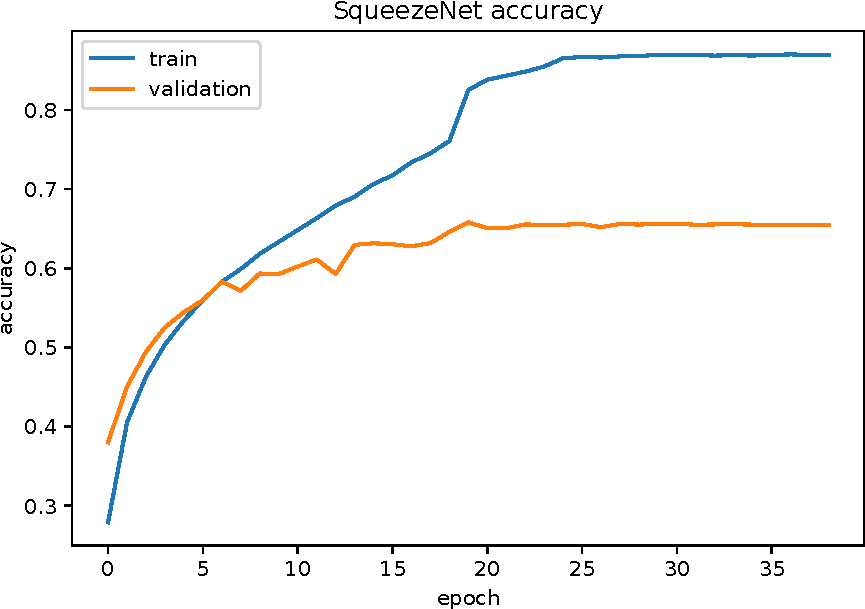
\includegraphics[width=0.45\columnwidth]{squeezeNet_cifar10_noaug.pdf}}
  \hfill
  \subfigure[accuracy for SqueezeNet with augmentation]{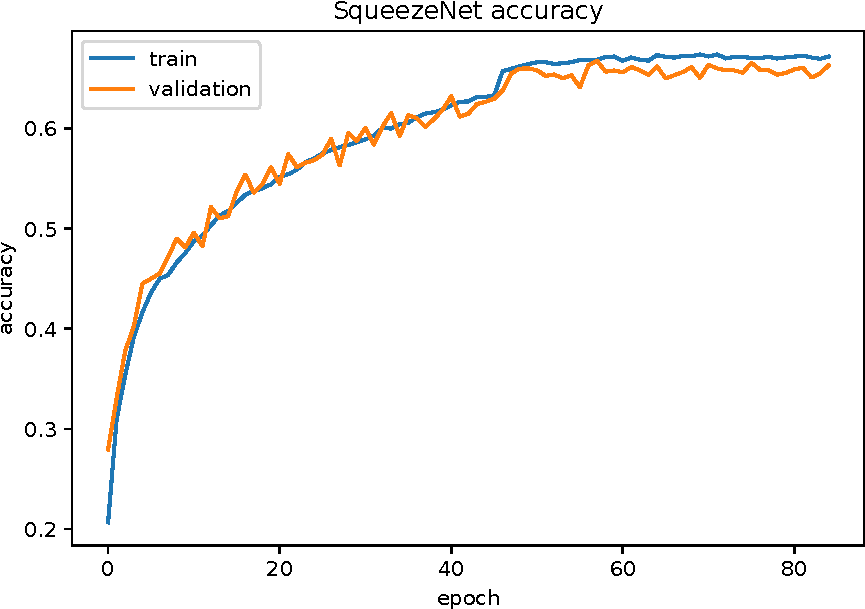
\includegraphics[width=0.45\columnwidth]{squeezeNet_cifar10_aug.pdf}}
  \hfill
\caption{Training-accuracy for SqueezeNet on the Cifar10 Dataset}
\label{rescnn::1}
\end{figure}

In figure \ref{rescnn::1} we can see the effect of the augmentation on the accuracy of the predictions while training. We have a clear overfitting of the CNN when not applying augmentation. This overfitting is largly decreased by applying the image-augmentation as can be seen in the figure. When applying the augmentation the accuracy of SqueezeNet on the Test-set increased from $65.21\%$ to $67.33\%$. Augmentation of the images has an influence on the efficiency of the parameter search for the Network. Without augmentation the optimal paramters are found after $6 \min$ and less than $40$ epochs, whereas augmentation causes the time for parameter search to increase to $46 \min$ and $84$ epochs. For the predition of the $313$ samples in the test-set SqueezeNet needs about $9 \text{s}$ 

\begin{figure}
\centering
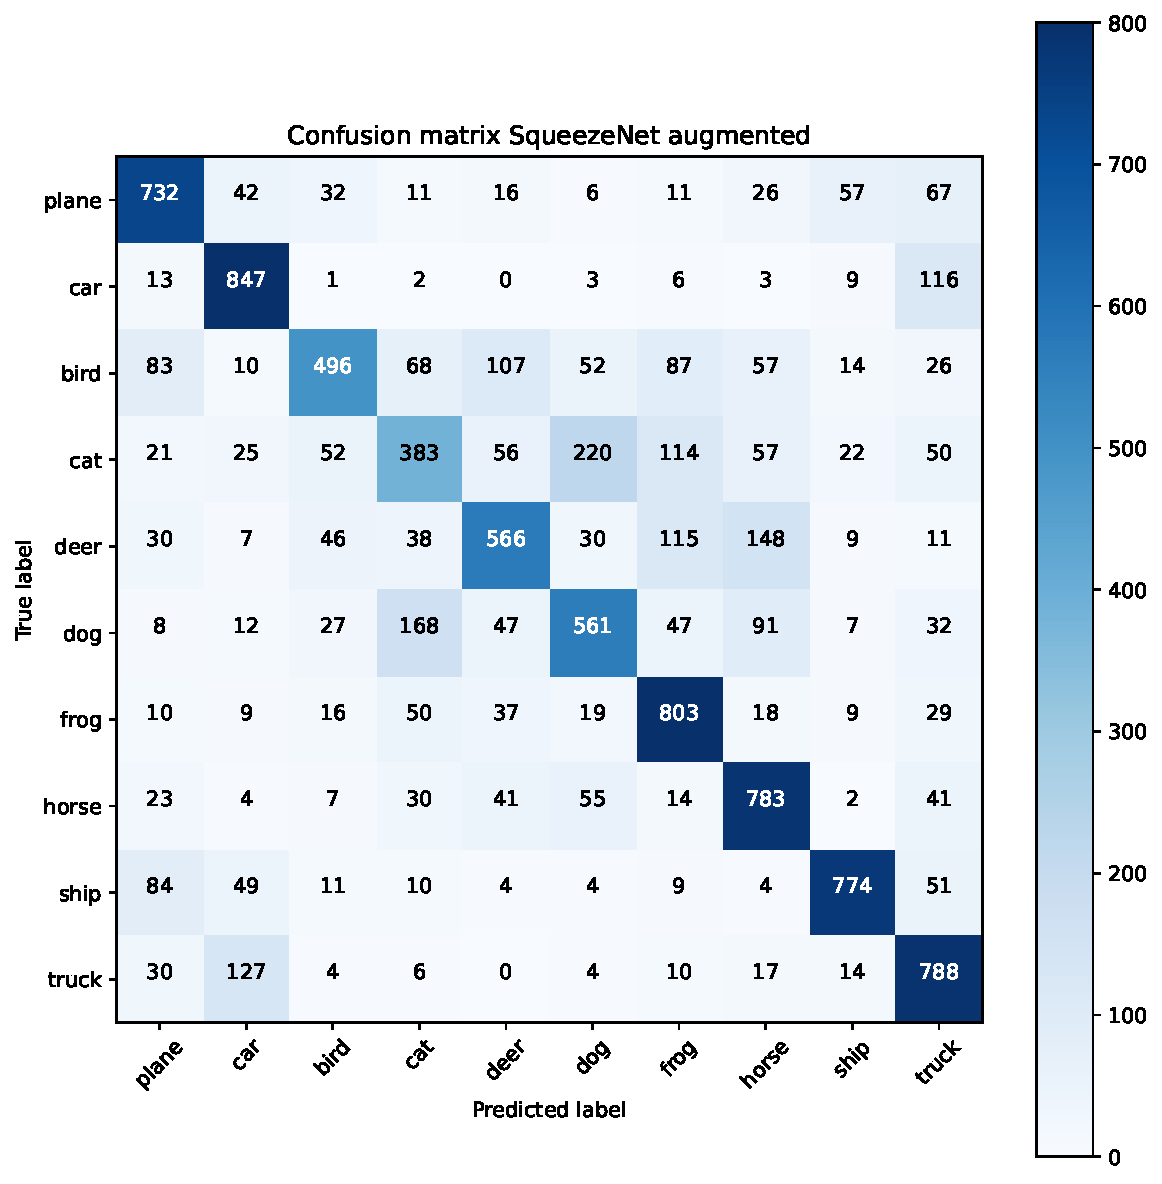
\includegraphics[width=0.5\columnwidth]{squeezeNet_cifar10_aug_confmat.pdf}
\caption{Confusion matrix for the SqueezeNet trained on the augmented Cifar10 Datase.}
\label{rescnn::2}
\end{figure}

In figure \ref{rescnn::2} we show the corresponding confusion matrix for the SqueezeNet trained on the augmented Cifar10 images. The most true positive labels are predicted for the car class with $847$ where we note that $127$ times a truch sample gets confused to be a car. The least true positive labels are predicted for cats with $383$ where this class often gets confused with the dog class. The most false negative preditions are made for the truck class with $423$ samples closely followed by the horse class with $421$ flsely predicted samples. This is due to the fact that Trucks are often confused with cars and horses are often confused with deers or dogs.

\subsection{Res50Net}
To create our wrapped Res50Net we stip off the top layers and replace that layer by a custom layer of $32\times 32 \times 3$ for reading our images. The output of the Res50Net gets fed into $3$ densle layers with $256, 128, 64$ neurons till it reaches the softmax layers for prediction. Note that our dense layers consist each at the top of a batch normalisation layer and the dense layers with a dropout of $50\%$ for regularisation purposes. For the Res50Net layers in our CNN we enable the training of the $168$ bottom layers and freeze the rest of them. By that we end up with a CNN that has in total $24.163.786$ parameters from which are $3.986.762$ trainable. For the transfer learning we apply the same image augmentation as for SqueezeNet.

\begin{figure}
\centering
\SetFigLayout{3}{2}
  \subfigure[accuracy for Res50Net without augmentation]{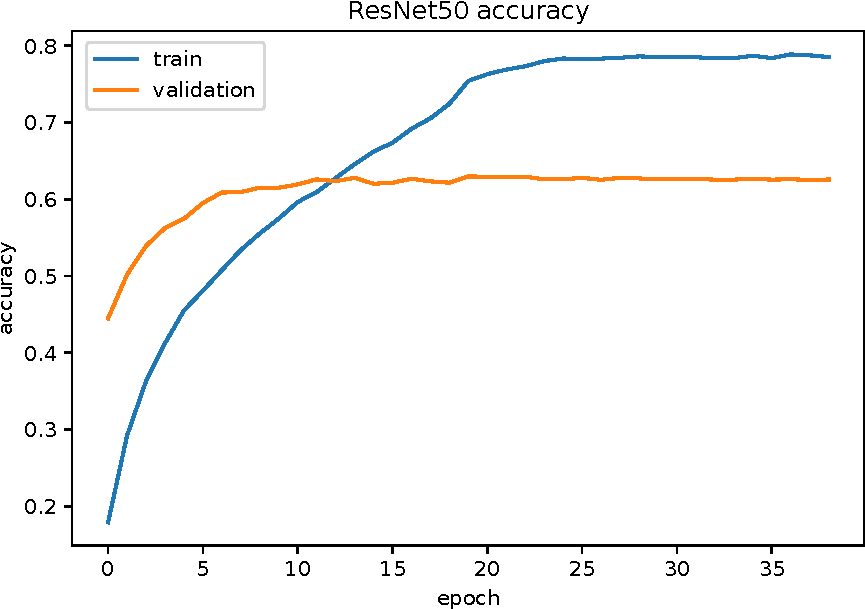
\includegraphics[width=0.45\columnwidth]{res50Net_cifar10_noaug.pdf}}
  \hfill
  \subfigure[accuracy for Res50Net with augmentation]{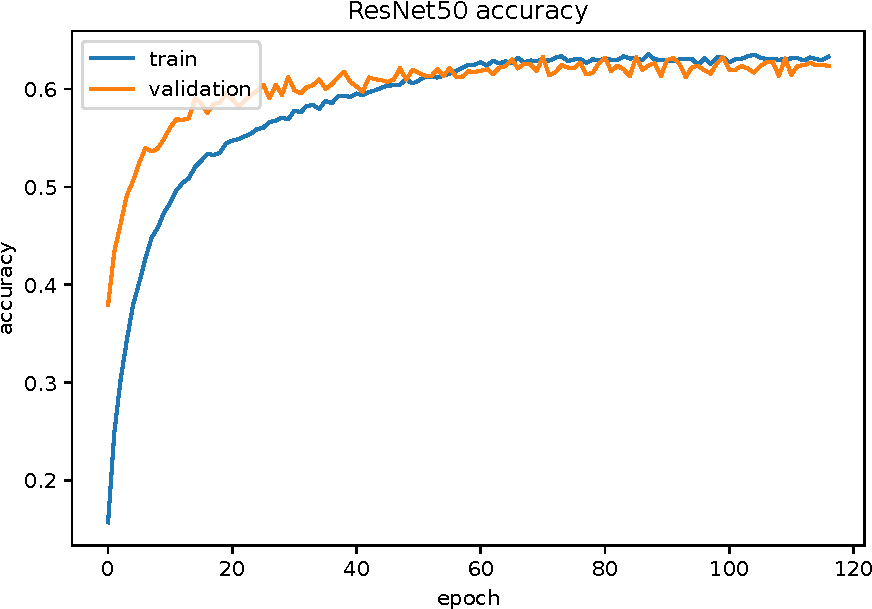
\includegraphics[width=0.45\columnwidth]{res50Net_cifar10_aug.pdf}}
  \hfill
\caption{Training-accuracy for Res50Net on the Cifar10 Dataset}
\label{rescnn::3}
\end{figure}

In figure \ref{rescnn::3} we show the accuracy while executing the transfer learning of Res50Net. Again without augmentation the CNN overfits till about $80\%$ accuracy on the trainset while the accuracy on the validation-set is $20\%$ lower. With augmentation we have diminished this effect and additionally improve the accuracy on the test-set from $62.16\%$ for no augmentation to $64.69\%$ with augmentation. The parameter-fitting for the augmented process took 117 epochs with a total time of $64 \min$ compared to that the parameter-fitting with no augmentation took $39$ epochs and about $10 \min$ in total. The evaluation on the testset took $38\text{s}$ which is more $4$ than longer than for the SqueezeNet.


\begin{figure}
\centering
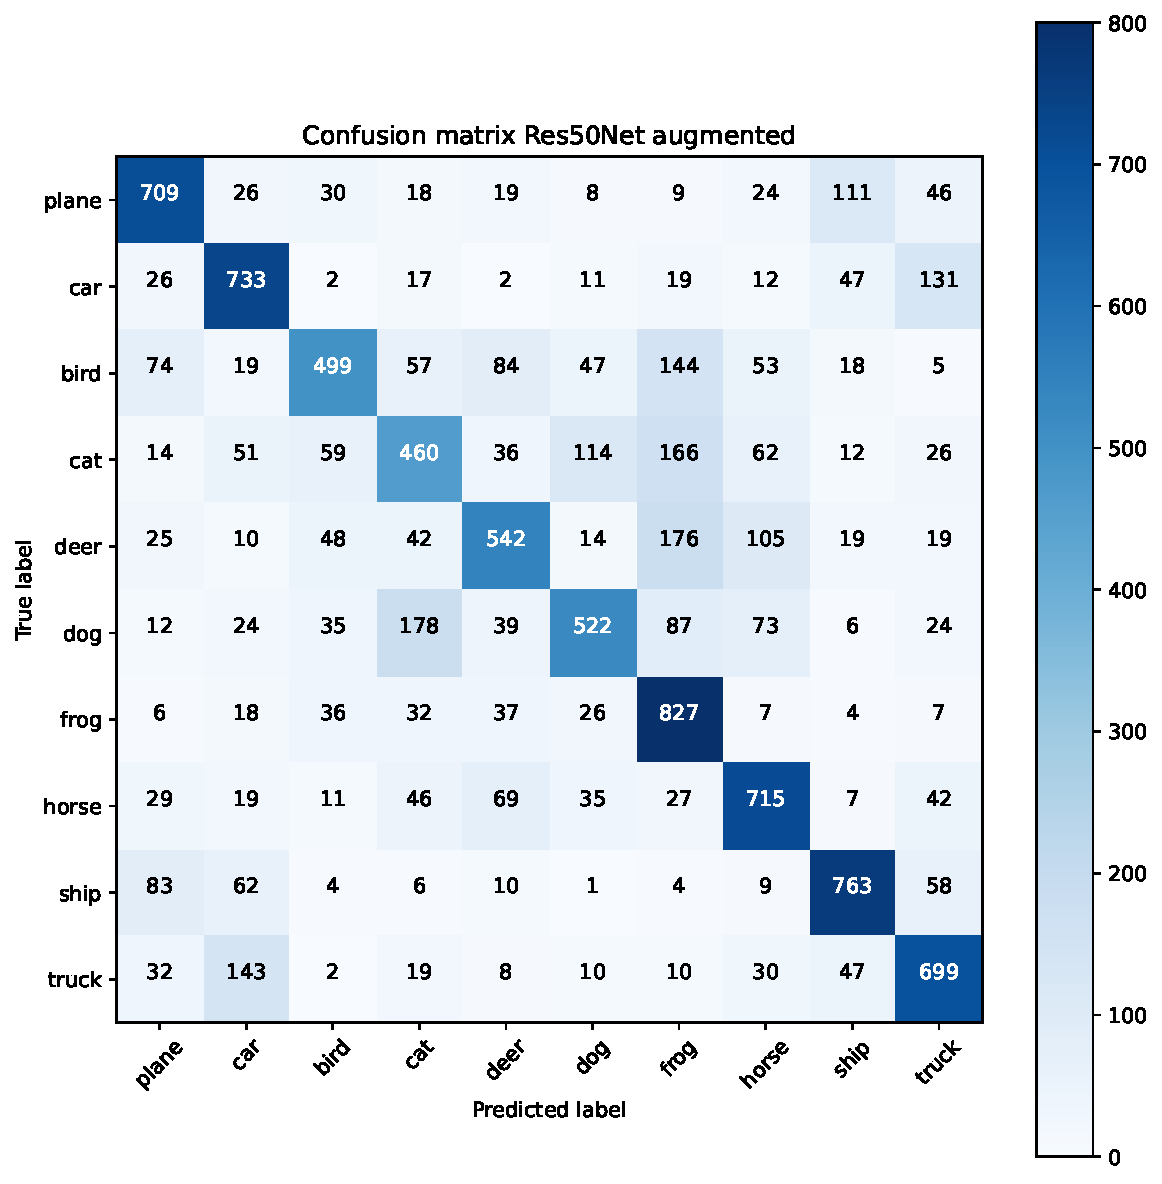
\includegraphics[width=0.5\columnwidth]{res50Net_cifar10_aug_confmat.pdf}
\caption{Confusion matrix for the SqueezeNet trained on the augmented Cifar10 Datase.}
\label{rescnn::4}
\end{figure}

In figure \ref{rescnn::4} the corresponding confusion matrix for the Res50Net trained on the augmented Cifar10 images is plotted. The most true positive predictions are made for the frog class with $827$. We also see that the frog class has aswell the most true negative predictions where it seems particularly hard for the CNN to differentiate it from other animals. The cat class with the one with lowest true positives at $460$, where we note that $148$ dogs get wrongly classified as cats. Also notable is that cars get often cofused as trucks and ships are often confused as planes. 


\subsubsection{Results}

  


\subsection{squeezNet}
For the second architecture we decided on unsing SqueezeNet \cite{iandola2016}. Squeezenet claims to have an accuracy equal to AlexNet but has a lot less parameters to learn.  
For SqeeuzeNet no weights are available, therefore we recreated the model and re-trained it. 



\subsubsection{Results}

%Bibliography
\newpage
\bibliographystyle{plain}
\bibliography{lib}

\end{document}
